\documentclass{oblivoir}

\usepackage{kotex}
\usepackage{amssymb}
\usepackage{amsmath}
\usepackage{graphicx}

\newenvironment{question}{ }{ \par\noindent\rule{\textwidth}{0.4pt} }

\graphicspath{ {./images/} }
\renewcommand{\figurename}{그림}
\renewcommand{\tablename}{표}
\newcommand{\figref}[1]{\figurename{} \ref{#1}}
\newcommand{\tabref}[1]{\tablename{} \ref{#1}}

\title{이산수학 (12744) 4번 레포트}
\author{순천향대학교 SW융합대학 컴퓨터소프트웨어공학과\\20223519 전한결}

\begin{document}

\maketitle

\begin{itemize}
    \item 작성자 --- SW융합대학 컴퓨터소프트웨어공학과 20223519 전한결
    \item 과목 --- 2023학년도 1학기 이산수학 (12744)
    \item 과제 제시일 --- 2023년 5월 9일
    \item 과제 마감일 --- 2023년 5월 16일
\end{itemize}

\pagebreak

\tableofcontents

\pagebreak

\section{Question 17}
\begin{question}
    관계 $R$에 대한 유향 그래프가 다음과 같을 때,
    물음에 답하라.

    \begin{figure}[h]
        \centering
        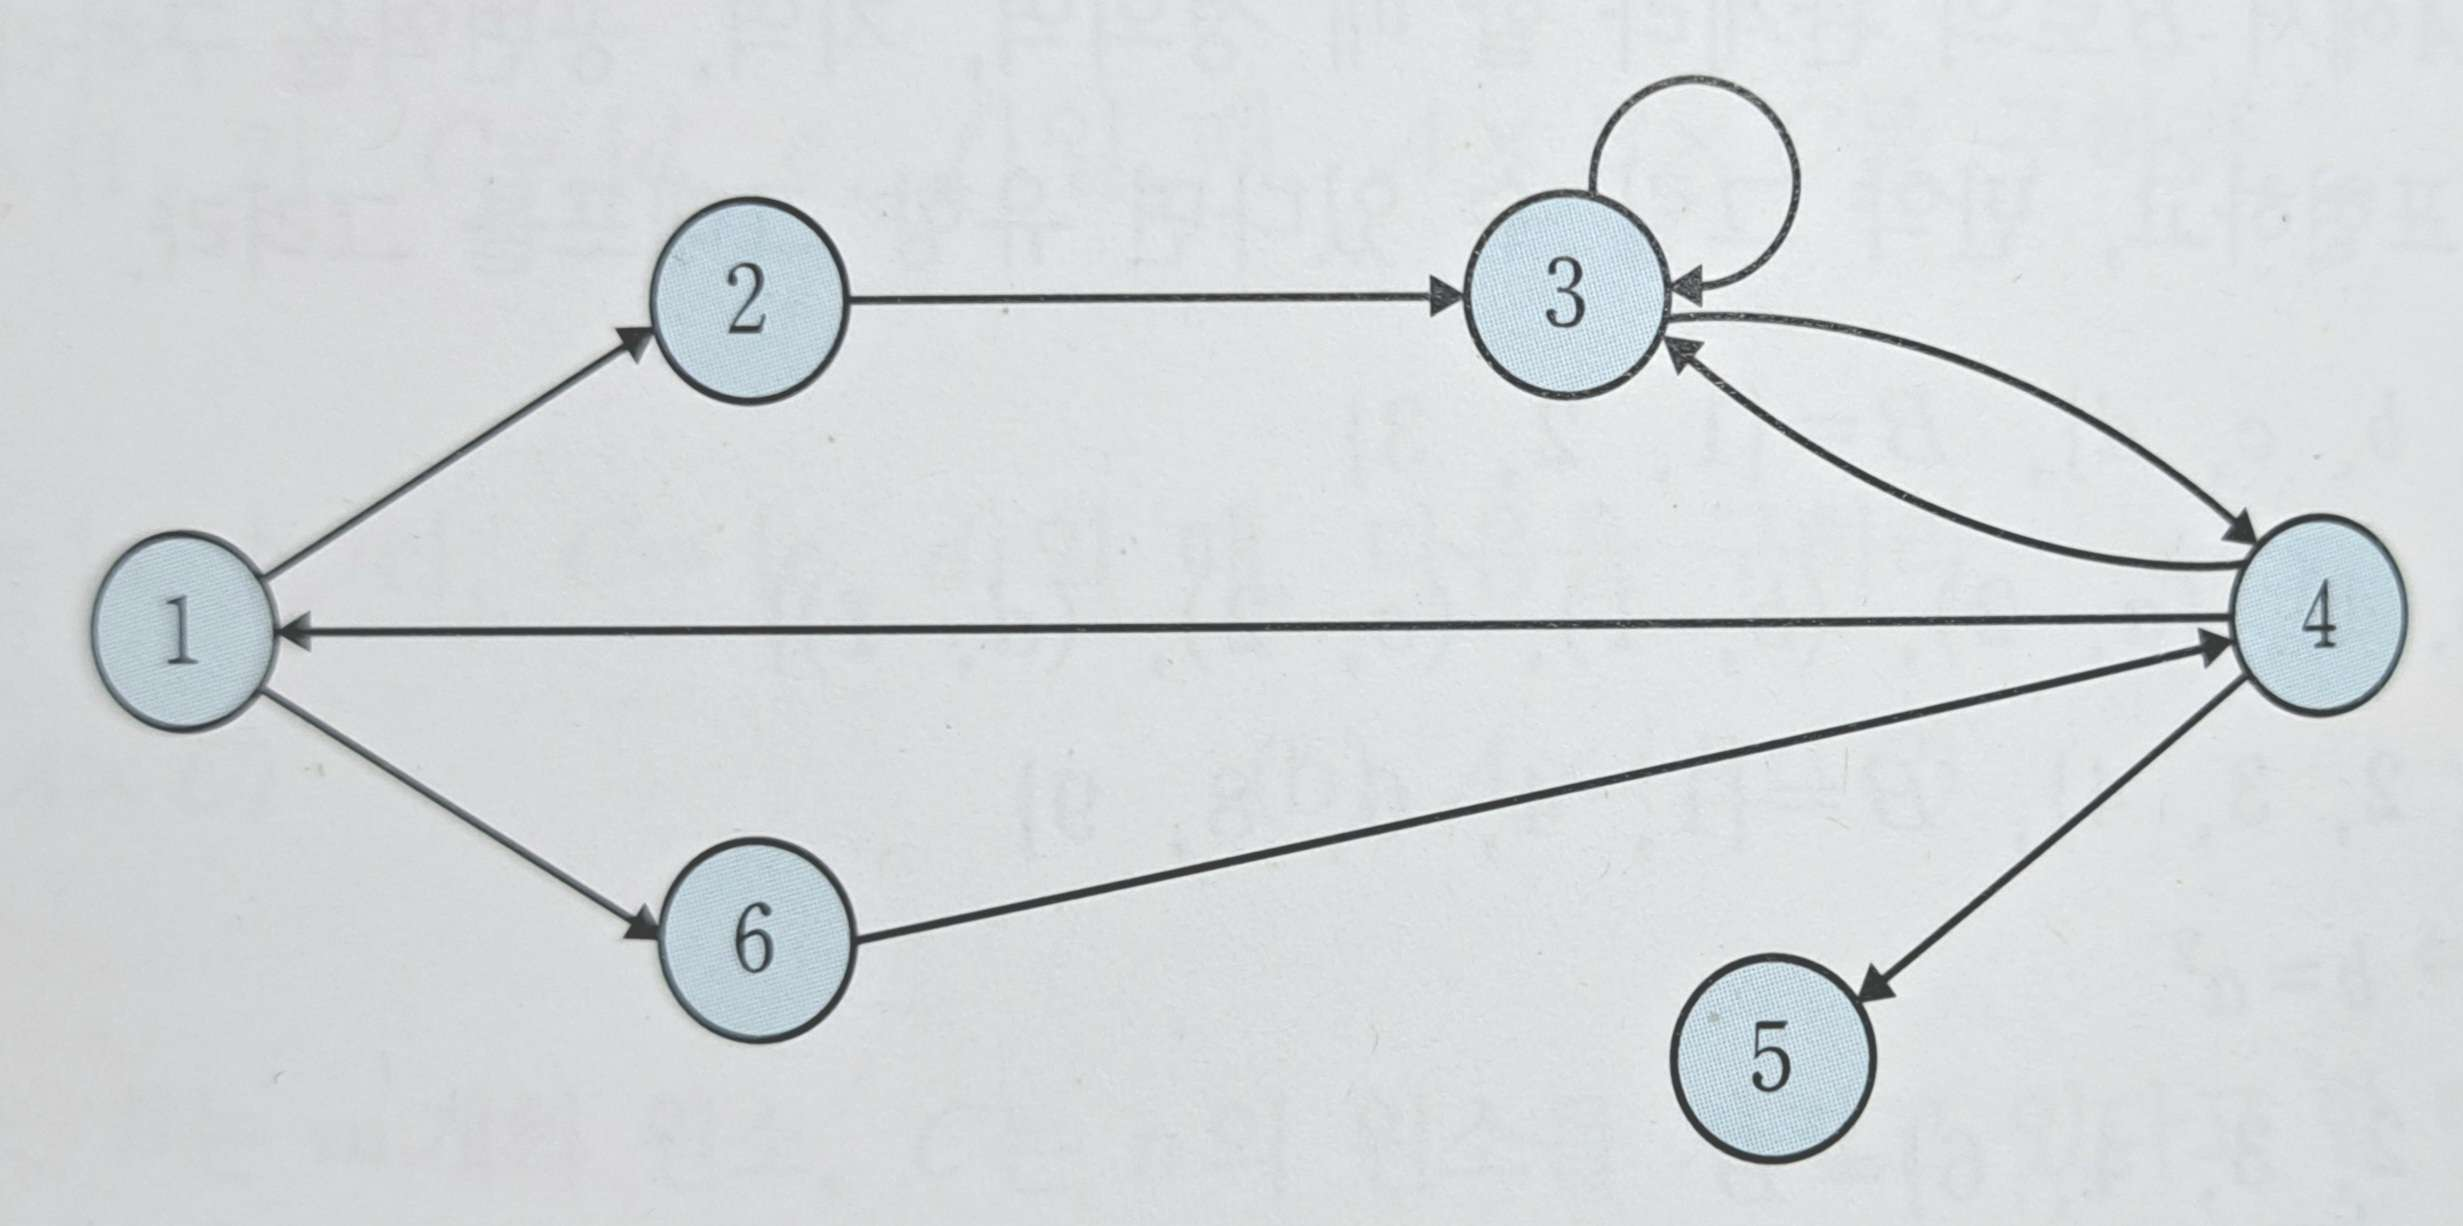
\includegraphics[width=10cm]{17}
        \caption{관계 $R$에 대한 유향 그래프}
        \label{fig:test_uno}
    \end{figure}

    \begin{enumerate}[(a)]
        \item 길이가 $1$인 경로들을 모두 나열하라.
        \item 정점 $2$에서 시작하여 길이가 $2$인 경로들을 모두 나열하라.
        \item 정점 $3$에서 시작하여 길이가 $3$인 경로들을 모두 나열하라.
        \item 정점 $2$에서 시작하는 모든 순환을 구하라.
        \item 정점 $6$에서 시작하는 모든 순환을 구하라.
        \item 길이가 $2$인 경로들을 모두 나열하라.
        \item 길이가 $3$인 경로들을 모두 나열하라.
        \item $R^2$의 유향 그래프를 그려라.
        \item $M_{R^2}$, $R^\infty$, $M_{R^\infty}$을 구하라.
    \end{enumerate}
\end{question}

\begin{equation}
    R = \left\{ (1,2), (1,6), (2,3), (3,3), (3,4), (4,1), (4,3), (4,5), (6,4) \right\}.
\end{equation}

\subsection{길이가 $1$인 경로들을 모두 나열하라.}

길이가 $1$인 경로란 어떤 정점에서 시작하여 인접한
다른 정점으로 끝나는 경로를 말한다.

$R$에 있는 모든 순서쌍은 시점과 종점을 나타내므로
그 자체로 길이가 $1$인 경로가 된다.

따라서 길이가 $1$인 경로를 모두 나열하면 다음과 같다.

\begin{equation}
    \{1,2\}, \{1,6\}, \{2,3\}, \{3,3\}, \{3,4\}, \{4,1\}, \{4,3\}, \{4,5\}, \{6,4\}.
\end{equation}

\subsection{정점 $2$에서 시작하여 길이가 $2$인 경로들을 모두 나열하라.}

정점 $2$에서 시작하는 길이가 $1$인 경로는 $\{2,3\}$뿐이다.
이때, $3$에서 시작하는 길이가 $1$인 경로는 $\{3,3\}, \{3,4\}$가 있다.

$2$에서 시작하는 경로는 종점이 $3$이고
$3$에서 시작하는 경로는 시점이 $3$이므로 두 경로를 합성할 수 있다.
두 경로를 합성하면 길이가 $2$인 경로로 다음을 얻을 수 있다.
\begin{equation}
    \{2,3,3\}, \{2,3,4\}.
\end{equation}

\subsection{정점 $3$에서 시작하여 길이가 $3$인 경로들을 모두 나열하라.}

정점 $3$에서 시작하는 길이가 $1$인 경로는 $\{3,3\}, \{3,4\}$이다.
정점 $4$에서 시작하는 길이가 $1$인 경로는 $\{4,1\}, \{4,3\}, \{4,5\}$이다.
정점 $1$에서 시작하는 길이가 $1$인 경로는 $\{1,2\}, \{1,6\}$이다.
정점 $5$에서 시작하는 길이가 $1$인 경로는 없다.

정점 $3$에서 시작하는 길이가 $2$인 경로는
각 길이가 $1$인 경로의 종점을 시점으로 하는 길이가 $1$인 경로를
합성하여 다음과 같이 얻어낼 수 있다.
\begin{equation}
    \{3,3,3\}, \{3,3,4\}, \{3,4,1\}, \{3,4,3\}, \{3,4,5\}.
\end{equation}
이때, 같은 방법으로 정점 $3$에서 시작하는 길이가 $3$인 경로는
각 길이가 $2$인 경로의 종점을 시점으로 하는 길이가 $1$인 경로를
합성하여 다음과 같이 얻어낼 수 있다.
\begin{equation}
    \begin{aligned}
        &\{3,3,3,3\}, \{3,3,4,1\}, \{3,3,4,3\}, \{3,3,4,5\}, \\
        &\{3,4,1,2\}, \{3,4,1,6\}, \{3,4,3,3\}, \{3,4,3,4\}.
    \end{aligned}
\end{equation}

\subsection{정점 $2$에서 시작하는 모든 순환을 구하라.}

$\{2,3,4,1,2\}$는 정점 $2$에서 시작하는 길이가 $4$인 순환이다.

이때, $3$에 $4$가 대응되고 $4$에 $3$이 대응되므로
경로 중간의 $3$은 $3,4,3$, $4$는 $4,3,4$로 바꿀 수 있다.
또한, $3$에 $3$ 자신이 대응되므로
경로 중간의 $3$은 $3,3$, $3,3,3$, $3,3,3,3$과 같이
3이 반복되는 부분으로 바꿀 수 있다.

이때, $3$ 또는 $4$와 바꿀 수 있는 경로의 수가 무한하므로
정점 $2$에서 시작하는 순환의 개수는 무한하다.
따라서 모든 순환을 구할 수 없다.

\subsection{정점 $6$에서 시작하는 모든 순환을 구하라.}

정점 $6$을 종점으로 하는 경로는 존재하지 않는다.
따라서 $6$에서 시작하고 $6$으로 끝나는 경로가 존재하지 않으므로
정점 $6$에서 시작하는 순환은 존재하지 않는다.

\subsection{길이가 $2$인 경로들을 모두 나열하라.}

길이가 $2$인 경로는 길이가 $1$인 경로의 종점을 시점으로 하는
길이가 $1$인 경로를 합성하여 다음과 같이 얻어낼 수 있다.

\begin{equation}\label{eq:2lp}
    \begin{aligned}
        &\{1,2,3\}, \{1,6,4\}, \{2,3,3\}, \{2,3,4\}, \{3,3,3\}, \\
        &\{3,3,4\}, \{3,4,1\}, \{3,4,3\}, \{3,4,5\}, \{4,1,2\}, \\
        &\{4,1,6\}, \{4,3,3\}, \{4,3,4\}, \{6,4,1\}, \{6,4,3\}, \\
        &\{6,4,5\}.
    \end{aligned}
\end{equation}

\subsection{길이가 $3$인 경로들을 모두 나열하라.}

길이가 $3$인 경로는 길이가 $1$인 경로의 종점을 시점으로 하는
길이가 $2$인 경로를 합성하여 얻어낼 수 있다.

길이가 $2$인 경로는 이미 \eqref{eq:2lp}에서 구했으므로
이것을 길이가 $1$인 경로와 합성하여 다음과 같이 얻어낼 수 있다.

\begin{equation}\label{eq:2lp}
    \begin{aligned}
        &\{1,2,3,3\}, \{1,2,3,4\}, \{1,6,4,1\}, \{1,6,4,3\}, \{1,6,4,5\}, \\
        &\{2,3,3,3\}, \{2,3,3,4\}, \{2,3,4,1\}, \{2,3,4,3\}, \{2,3,4,5\}, \\
        &\{3,3,3,3\}, \{3,3,3,4\}, \{3,3,4,1\}, \{3,3,4,3\}, \{3,3,4,5\}, \\
        &\{3,4,1,2\}, \{3,4,1,6\}, \{3,4,3,3\}, \{3,4,3,4\}, \{4,1,2,3\}, \\
        &\{4,1,6,4\}, \{4,3,3,3\}, \{4,3,3,4\}, \{4,3,4,1\}, \{4,3,4,3\}, \\
        &\{4,3,4,5\}, \{6,4,1,2\}, \{6,4,1,6\}, \{6,4,3,3\}, \{6,4,3,4\}.
    \end{aligned}
\end{equation}

\subsection{$R^2$의 유향 그래프를 그려라.}

$R^2$는 $R$을 두 번 합성한 것이므로
길이가 $2$인 경로들을 모두 나열한 \eqref{eq:2lp}에서
시점과 종점을 왼쪽과 오른쪽 요소로 하는 순서쌍의 집합으로 표현되는
대응 관계이다.
이는 다음과 같다.
\begin{equation}
    \begin{aligned}
        R^2 = \{
            &(1,3), (1,4), (2,3), (2,4), (3,1), (3,3), (3,4), (3,5), \\
            &(4,2), (4,3), (4,4), (4,6), (6,1), (6,3), (6,5)
        \}.
    \end{aligned}
\end{equation}

이것을 유향 그래프로 나타내면 \figref{fig:17-8}과 같다.

\begin{figure}[h]
    \centering
    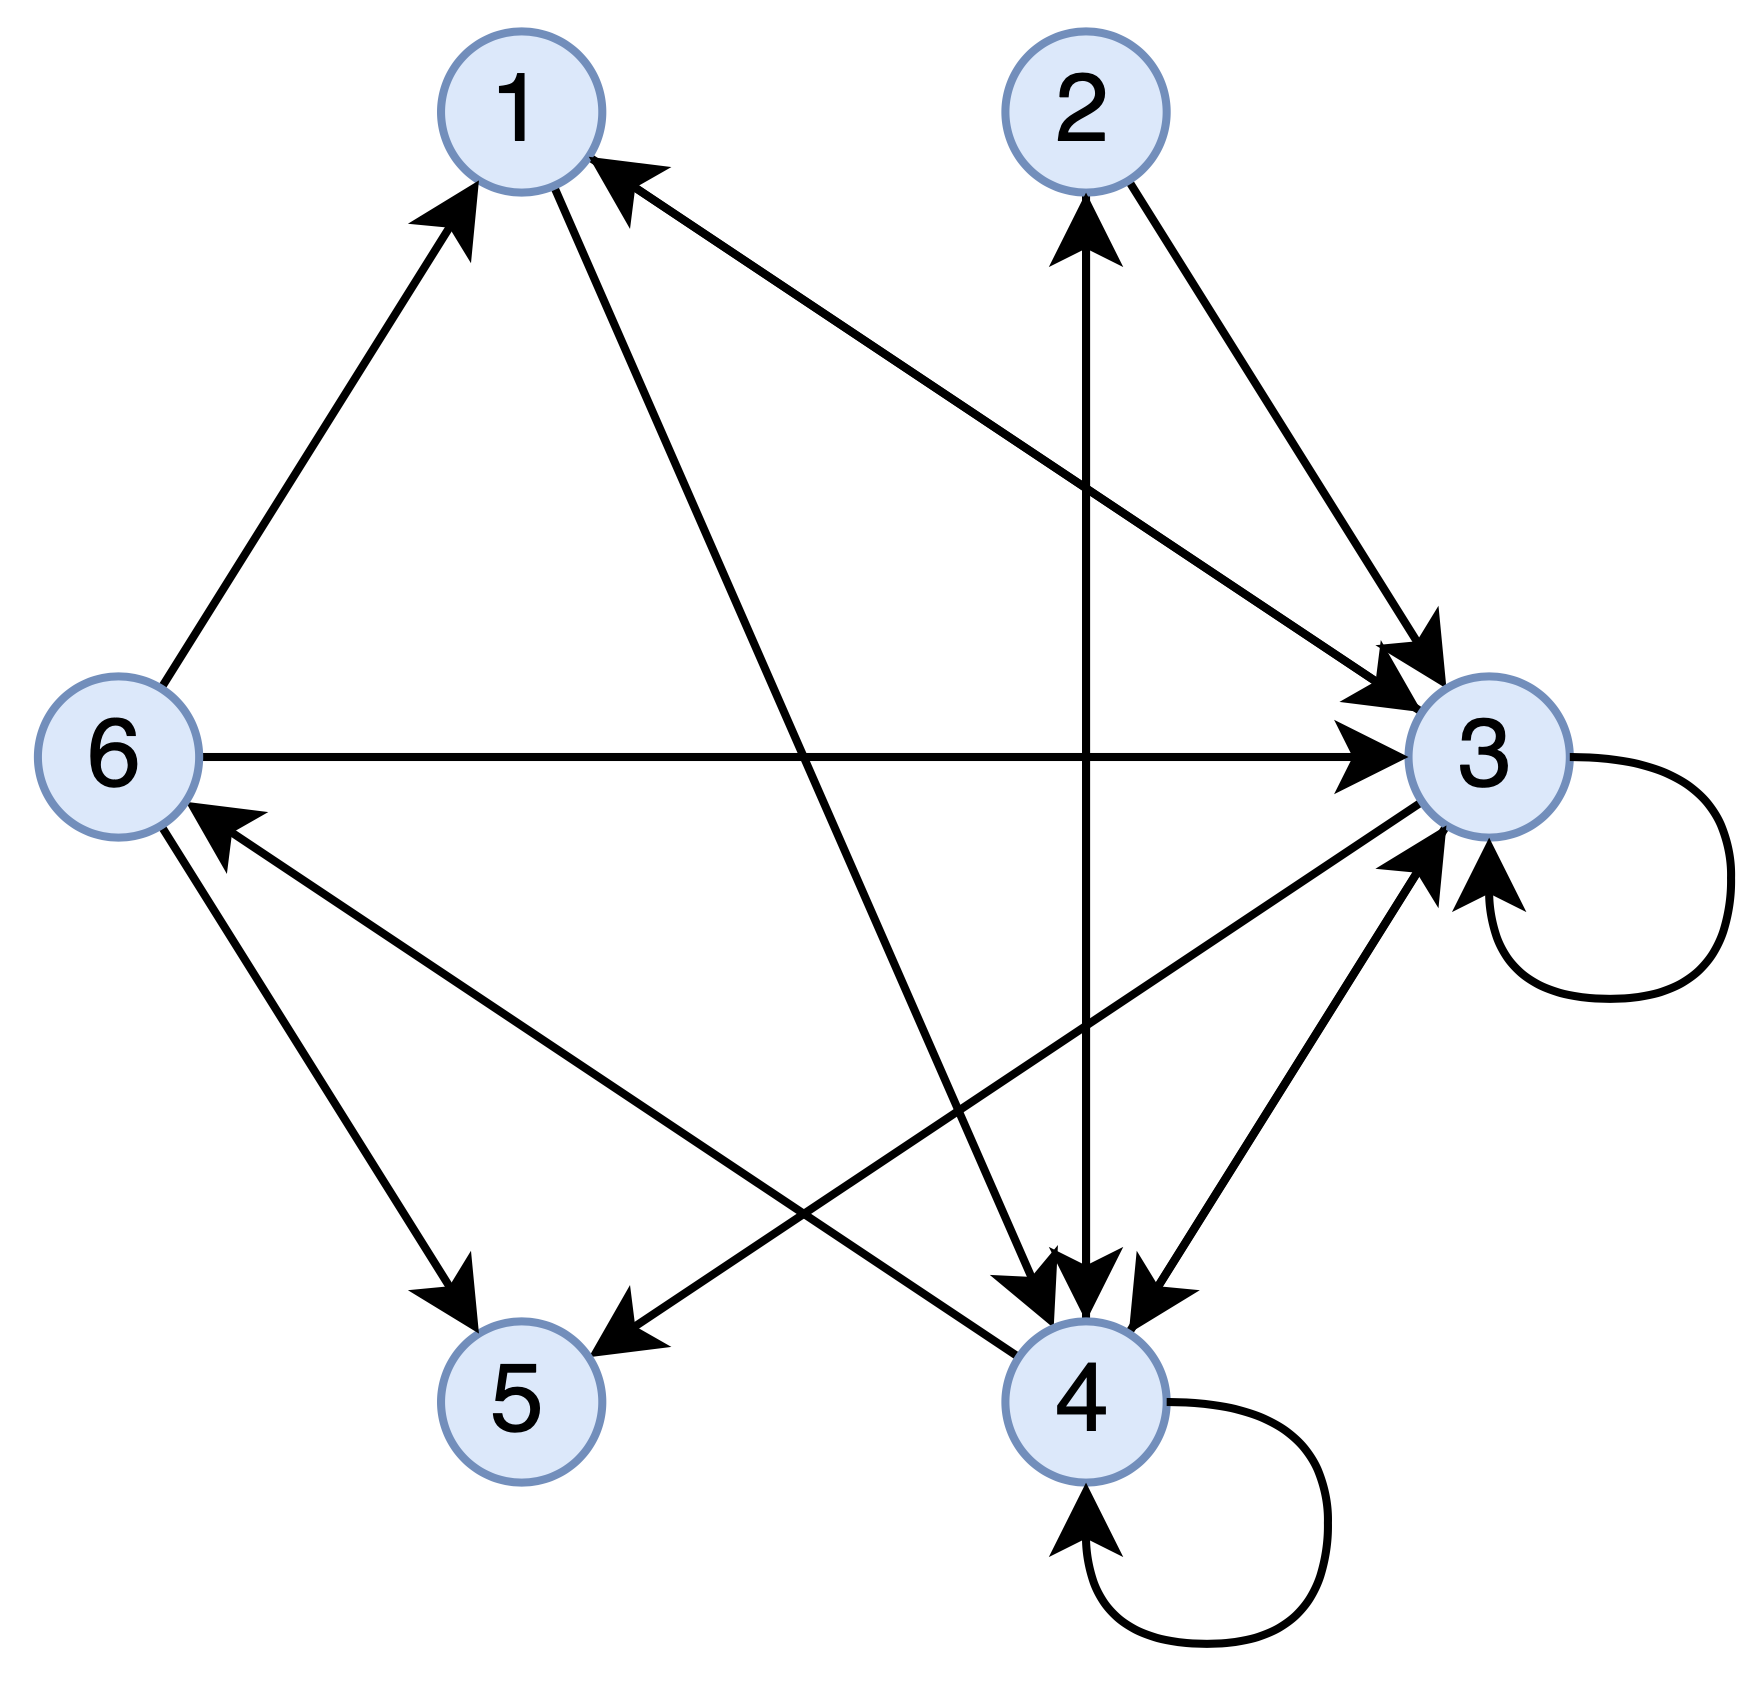
\includegraphics[width=5cm]{17-8}
    \caption{$R^2$의 유향 그래프}
    \label{fig:17-8}
\end{figure}

\subsection{$M_{R^2}$, $R^\infty$, $M_{R^\infty}$을 구하라.}

$M_{R^2}$는 $R^2$의 행렬 표현이다.
이는 $R^2$의 요소의 첫 번째 요소를 행, 두 번째 요소를 열로 하는
행렬의 해당 위치에 $1$을 채우고 나머지 위치에 $0$을 채운 것이다.
\begin{equation}
    M_{R^2} = \left[ \begin{cases}
        1,& \text{if } (i,j) \in R^2 \\
        0,& \text{otherwise}
    \end{cases} \right] = \begin{bmatrix}
        0 & 0 & 1 & 1 & 0 & 0 \\
        0 & 0 & 1 & 1 & 0 & 0 \\
        1 & 0 & 1 & 1 & 1 & 0 \\
        0 & 1 & 1 & 1 & 0 & 1 \\
        0 & 0 & 0 & 0 & 0 & 0 \\
        1 & 0 & 1 & 0 & 1 & 0
    \end{bmatrix}.
\end{equation}

$R^\infty$는 임의의 정점에서 출발하여
임의의 길이인 경로를 따라가는 것이 가능한지 여부를 나타내는
대응 관계이다.
이는 가능한 경우의 수를 직접 하나하나 계산해보면 알 수 있다.

\begin{itemize}
    \item $(1,1)$의 경우 $\{1,2,3,4,1\}$을 따라갈 수 있으므로 가능하다.
    \item $(1,2)$의 경우 $\{1,2\}$을 따라갈 수 있으므로 가능하다.
    \item $(1,3)$의 경우 $\{1,2,3\}$을 따라갈 수 있으므로 가능하다.
    \item $(1,4)$의 경우 $\{1,2,3,4\}$을 따라갈 수 있으므로 가능하다.
    \item $(1,5)$의 경우 $\{1,4,5\}$을 따라갈 수 있으므로 가능하다.
    \item $(1,6)$의 경우 $\{1,6\}$을 따라갈 수 있으므로 가능하다.
    \item $(2,1)$의 경우 $\{2,3,4,1\}$을 따라갈 수 있으므로 가능하다.
    \item $(2,2)$의 경우 $\{2,3,4,1,2\}$을 따라갈 수 있으므로 가능하다.
    \item $(2,3)$의 경우 $\{2,3\}$을 따라갈 수 있으므로 가능하다.
    \item $(2,4)$의 경우 $\{2,3,4\}$을 따라갈 수 있으므로 가능하다.
    \item $(2,5)$의 경우 $\{2,3,4,5\}$을 따라갈 수 있으므로 가능하다.
    \item $(2,6)$의 경우 $\{2,3,4,1,6\}$을 따라갈 수 있으므로 가능하다.
    \item $(3,1)$의 경우 $\{3,4,1\}$을 따라갈 수 있으므로 가능하다.
    \item $(3,2)$의 경우 $\{3,4,1,2\}$을 따라갈 수 있으므로 가능하다.
    \item $(3,3)$의 경우 $\{3,3\}$을 따라갈 수 있으므로 가능하다.
    \item $(3,4)$의 경우 $\{3,4\}$을 따라갈 수 있으므로 가능하다.
    \item $(3,5)$의 경우 $\{3,4,5\}$을 따라갈 수 있으므로 가능하다.
    \item $(3,6)$의 경우 $\{3,4,1,6\}$을 따라갈 수 있으므로 가능하다.
    \item $(4,1)$의 경우 $\{4,1\}$을 따라갈 수 있으므로 가능하다.
    \item $(4,2)$의 경우 $\{4,1,2\}$을 따라갈 수 있으므로 가능하다.
    \item $(4,3)$의 경우 $\{4,3\}$을 따라갈 수 있으므로 가능하다.
    \item $(4,4)$의 경우 $\{4,3,4\}$을 따라갈 수 있으므로 가능하다.
    \item $(4,5)$의 경우 $\{4,5\}$을 따라갈 수 있으므로 가능하다.
    \item $(4,6)$의 경우 $\{4,1,6\}$을 따라갈 수 있으므로 가능하다.
    \item $(5,1)$의 경우 $5$에서 $1$로 끝나는 경로가 없으므로 불가능하다.
    \item $(5,2)$의 경우 $5$에서 $2$로 끝나는 경로가 없으므로 불가능하다.
    \item $(5,3)$의 경우 $5$에서 $3$로 끝나는 경로가 없으므로 불가능하다.
    \item $(5,4)$의 경우 $5$에서 $4$로 끝나는 경로가 없으므로 불가능하다.
    \item $(5,5)$의 경우 $5$에서 $5$로 끝나는 경로가 없으므로 불가능하다.
    \item $(5,6)$의 경우 $5$에서 $6$로 끝나는 경로가 없으므로 불가능하다.
    \item $(6,1)$의 경우 $\{6,4,1\}$을 따라갈 수 있으므로 가능하다.
    \item $(6,2)$의 경우 $\{6,4,1,2\}$을 따라갈 수 있으므로 가능하다.
    \item $(6,3)$의 경우 $\{6,4,1,2,3\}$을 따라갈 수 있으므로 가능하다.
    \item $(6,4)$의 경우 $\{6,4\}$을 따라갈 수 있으므로 가능하다.
    \item $(6,5)$의 경우 $\{6,4,5\}$을 따라갈 수 있으므로 가능하다.
    \item $(6,6)$의 경우 $\{6,4,1,6\}$을 따라갈 수 있으므로 가능하다.
\end{itemize}
따라서 $R^\infty$는 다음과 같다.
\begin{equation}\label{eq:R_infty}
    \begin{aligned}
        R^\infty = \{
            &(1,1), (1,2), (1,3), (1,4), (1,5), (1,6),\\
            &(2,1), (2,2), (2,3), (2,4), (2,5), (2,6),\\
            &(3,1), (3,2), (3,3), (3,4), (3,5), (3,6),\\
            &(4,1), (4,2), (4,3), (4,4), (4,5), (4,6),\\
            &(6,1), (6,2), (6,3), (6,4), (6,5), (6,6)\}.
    \end{aligned}
\end{equation}

\eqref{eq:R_infty}를 통해 $R^\infty$을 행렬로 나타내면 다음과 같다.
\begin{equation}
    M_{R^\infty} = \begin{bmatrix}
        1 & 1 & 1 & 1 & 1 & 1\\
        1 & 1 & 1 & 1 & 1 & 1\\
        1 & 1 & 1 & 1 & 1 & 1\\
        1 & 1 & 1 & 1 & 1 & 1\\
        0 & 0 & 0 & 0 & 0 & 0\\
        1 & 1 & 1 & 1 & 1 & 1
    \end{bmatrix}.
\end{equation}

\section{Question 26}
\begin{question}
    $A$와 $A$에 관한 관계 $R$이 다음과 같을 때
    $R$이 반사, 비반사, 대칭, 비대칭, 반대칭, 또는 추이 관계인가를 결정하라.

    \begin{enumerate}[(a)]
        \item $A = \mathbb Z,\ R = \left\{ (a,b) \in A \times A \mid a \leq b + 1 \right\}$
        \item $A = \mathbb Z^+,\ R = \left\{ (a,b) \in A \times A \mid |a-b| \leq 2 \right\}$
        \item $A = \mathbb Z,\ R = \left\{ (a,b) \in A \times A \mid a + b\textrm{는 짝수} \right\}$
        \item $A = \mathbb Z,\ R = \left\{ (a,b) \in A \times A \mid |a-b| = 2 \right\}$
        \item $A = \textrm{모든 실수의 집합},\ R = \left\{ (a,b) \in A \times A \mid a^2 + b^2 = 4 \right\}$
    \end{enumerate}
\end{question}

\subsection{$A = \mathbb Z,\ R = \left\{ (a,b) \in A \times A \mid a \leq b + 1 \right\}$}

\paragraph{반사 관계}
$\forall x \in A$에 대해
\begin{equation}\label{eq:x01}
    \begin{aligned}
        x &\leq x + 1 \\
        0 &\leq 1
    \end{aligned}
\end{equation}
은 참이므로 $x \mathrel R x$이다. 따라서 $R$은 반사 관계이다.

\paragraph{비반사 관계}
\eqref{eq:x01}에 의해 $\forall x \in A,\ x \mathrel R x$이므로
$R$은 비반사 관계가 아니다.

\paragraph{대칭 관계}
$x = 1,\ y = 3$일 때
\begin{equation}\label{eq:xy13_1}
    \begin{aligned}
        x &\leq y + 1 \\
        1 &\leq 3 + 1 = 4
    \end{aligned}
\end{equation}
는 참이므로 $x \mathrel R y$이다.
하지만 이때
\begin{equation}\label{eq:xy13_2}
    \begin{aligned}
        y &\leq x + 1 \\
        3 &\leq 1 + 1 = 2
    \end{aligned}
\end{equation}
는 거짓이므로 $y \not \mathrel R x$이다.
$A \times A$의 임의의 원소 $(y,x) = (3,1)$에 대해 $y \not \mathrel R x$이므로
$R$은 대칭 관계가 아니다.

\paragraph{비대칭 관계}
$x = 1,\ y = 2$에 대해
\begin{equation}\label{eq:xy12_1}
    \begin{aligned}
        x &\leq y + 1 \\
        1 &\leq 2 + 1 = 3
    \end{aligned}
\end{equation}
는 참이므로 $x \mathrel R y$이다.
이때
\begin{equation}\label{eq:xy12_2}
    \begin{aligned}
        y &\leq x + 1 \\
        2 &\leq 1 + 1 = 2
    \end{aligned}
\end{equation}
역시 참이므로 $y \mathrel R x$이다.
$A$의 임의의 원소 $x = 1,\ y = 2$에 대해
$x \mathrel R y \Rightarrow y \mathrel R x$이므로
$R$은 비대칭 관계가 아니다.

\paragraph{반대칭 관계}
\eqref{eq:xy12_1}과 \eqref{eq:xy12_2}를 통해
$A$의 임의의 원소 $x = 1,\ y = 2$에 대해
$x \mathrel R y$이고 $y \mathrel R x$이다.
$x \neq y \Rightarrow x \mathrel R y \wedge y \mathrel R x$이므로
$(x,y)$는 반대칭관계의 조건에 대한 반례가 된다.
따라서 $R$은 반대칭 관계가 아니다.

\paragraph{추이 관계}
$x = 2,\ y = 1,\ z = 0$이라면
\eqref{eq:xy12_2}을 통해 $x \mathrel R y$이고,
\begin{equation}
    \begin{aligned}
        y &\leq z + 1 \\
        1 &\leq 0 + 1 = 1
    \end{aligned}
\end{equation}
가 참이므로 $y \mathrel R z$이다.
하지만
\begin{equation}
    \begin{aligned}
        x &\leq z + 1 \\
        2 &\leq 0 + 1 = 1
    \end{aligned}
\end{equation}
이므로 $x \not \mathrel R z$이다.
즉, $(x,y,z) = (2,1,0)$은 추이 관계의 조건에 대한 반례이므로
$R$은 추이 관계가 아니다.

따라서 $R$은 반사 관계이지만 비반사 관계가 아니며
대칭 관계가 아니고 비대칭 관계가 아니고 반대칭 관계가 아니고
추이 관계가 아니다.

\subsection{$A = \mathbb Z^+,\ R = \left\{ (a,b) \in A \times A \mid |a-b| \leq 2 \right\}$}

\paragraph{반사 관계}
$\forall x \in A$에 대해
\begin{equation}\label{eq:x2}
    |x - x| = 0 \leq 2
\end{equation}
가 참이므로 $x \mathrel R x$이다.
따라서 $R$은 반사 관계이다.

\paragraph{비반사 관계}
\eqref{eq:x2}에 의해 $\forall x \in A,\ x \mathrel R x$이므로
$R$은 비반사 관계가 아니다.

\paragraph{대칭 관계}
$\forall x, y \in A,\ |x-y| \leq 2$라면 $|y-x| = |x - y| \leq 2$이므로
$x \mathrel R y \Rightarrow y \mathrel R x$이다.
따라서 $R$은 대칭 관계이다.

\paragraph{비대칭 관계}
$x = 1,\ y = 2$에 대해
\begin{equation}\label{eq:xy12a_1}
    |x - y| = |1 - 2| = |-1| = 1 \leq 2
\end{equation}
이므로 $x \mathrel R y$이고
\begin{equation}\label{eq:xy12a_2}
    |y - x| = |2 - 1| = |1| = 1 \leq 2
\end{equation}
이므로 $y \mathrel R x$이다.
$A$의 임의의 원소 $x,y$에 대해 $x \mathrel R y \wedge y \mathrel R x$이므로
$(x,y)$는 비대칭 관계의 조건에 대한 반례가 된다.
따라서 $R$은 비대칭 관계가 아니다.

\paragraph{반대칭 관계}
$x = 1,\ y = 2$, 즉 $x \neq y$일 때
\eqref{eq:xy12a_1}과 \eqref{eq:xy12a_2}에 의해
$x \mathrel R y \wedge y \mathrel R x$이므로
$(x,y) = (1,2)$는 반대칭 관계의 조건에 대한 반례가 된다.
따라서 $R$은 반대칭 관계가 아니다.

\paragraph{추이 관계}
$x = 0,\ y = 2,\ z = 4$라면
\begin{align}
    |x - y| &= |0 - 2| = |-2| = 2 \leq 2 \\
    |y - z| &= |2 - 4| = |-2| = 2 \leq 2
\end{align}
이므로 $x \mathrel R y$이고 $y \mathrel R z$이다.
하지만
\begin{equation}
    |x - z| = |0 - 4| = |-4| = 4 \leq 2
\end{equation}가 거짓이므로
$x \not \mathrel R z$이다.
따라서 $(x,y,z) = (0,2,4)$는 추이 관계의 조건에 대한 반례이므로
$R$은 추이 관계가 아니다.

따라서 $R$은 반사 관계이고 대칭 관계이지만
비반사 관계가 아니며 비대칭 관계가 아니고 반대칭 관계가 아니고
추이 관계가 아니다.

\subsection{$A = \mathbb Z,\ R = \left\{ (a,b) \in A \times A \mid a + b\textrm{는 짝수} \right\}$}

\paragraph{반사 관계}
$\forall x \in A$에 대해 $x + x = 2x$이므로 $x + x$는 짝수이다.
따라서 $x \mathrel R x$이므로 $R$은 반사 관계이다.

\paragraph{비반사 관계}
$\forall x \in A$에 대해 $x \mathrel R x$이므로
$R$은 비반사 관계가 아니다.

\paragraph{대칭 관계}
$\forall x,y \in A$에 대해 $x + y$가 짝수이면 $x \mathrel R y$이다.
이때, $y + x = x + y$이므로 $y + x$ 역시 짝수가 된다.
따라서 $y \mathrel R x$이다.
따라서 $R$은 대칭 관계이다.

\paragraph{비대칭 관계}
$x = 1,\ y = 1$일 때 $x \mathrel R y$이고 $y \mathrel R x$이므로
$(x,y) = (1,1)$은 비대칭관계의 조건에 대한 반례가 된다.
따라서 $R$은 비대칭 관계가 아니다.

\paragraph{반대칭 관계}
$x = 0,\ y = 2$일 때 $x + y = 0 + 2 = 2$이고 $2$는 짝수이므로 $x \mathrel R y$이다.
또한
\begin{equation}
    y + x = 2 + 0 = 2
\end{equation}이고 $2$는 짝수이므로 $y \mathrel R x$이다.
따라서 $x \mathrel R y \wedge y \mathrel R x$이고,
이것은 반대칭 관계에 대한 조건의 반례가 된다.
따라서 $R$은 반대칭 관계가 아니다.

\paragraph{추이 관계}
$x_1,x_2$가 모두 홀수인 경우 $x_1 + x_2$는 짝수이므로 $x_1 \mathrel R x_2$이다.
만약 $x$가 홀수라면 $x_2 + x$도 짝수이므로 $x_2 \mathrel R x$가 된다.
이때, $x_1$ 역시도 홀수이므로 $x_1 + x$는 짝수가 되어 $x_1 \mathrel R x$이다.

$y_1,y_2$가 모두 짝수인 경우 $y_1 + y_2$는 짝수이므로 $y_1 \mathrel R y_2$이다.
만약 $y$가 짝수라면 $y_2 + y$도 짝수이므로 $y_2 \mathrel R y$가 된다.
이때, $y_1$ 역시도 짝수이므로 $y_1 + y$는 짝수가 되어 $y_1 \mathrel R y$이다.

홀수와 짝수가 서로 좌·우변에 위치하는 경우에는
$R$을 만족하지 않으므로 추이 관계에서 다루지 않는다.

모든 경우에 대해서 추이 관계의 조건을 만족하므로 $R$은 추이 관계이다.

따라서 $R$은 반사 관계이고 대칭 관계이고 추이 관계이지만
비반사 관계가 아니고 비대칭 관계가 아니고 반대칭 관계가 아니다.

\subsection{$A = \mathbb Z,\ R = \left\{ (a,b) \in A \times A \mid |a-b| = 2 \right\}$}

\paragraph{반사 관계}
$\forall x \in A$에 대해,
\begin{equation}
    |x - x| = |0| = 0 \neq 2
\end{equation}이므로
$x \not \mathrel R x$이다.
따라서 $R$은 반사관계가 아니다.

\paragraph{비반사 관계}
$\forall x \in A$에 대해,
\begin{equation}
    |x - x| = |0| = 0 \neq 2
\end{equation}이므로
$x \not \mathrel R x$이다.
따라서 $R$은 비반사관계이다.

\paragraph{대칭 관계}
$\forall x, y \in A$에 대해 $|x - y| = 2$라면 $x \mathrel R y$이다.
이때,
\begin{equation}
    |y - x| = |x - y| = 2
\end{equation}
이므로 $f \mathrel R x$이다.
따라서 $R$은 대칭 관계이다.

\paragraph{비대칭 관계}
$\forall x, y \in A$에 대해 $|x - y| = 2$라면 $x \mathrel R y$이다.
따라서 $R$은 비대칭 관계가 아니다.

\paragraph{반대칭 관계}
$x = 1,\ y = 3$이라면
\begin{equation}
    |x - y| = |1 - 3| = |-2| = 2
\end{equation}
이므로 $x \mathrel R y$이다.
또한,
\begin{equation}
    |y - x| = |x - y| = 2
\end{equation}
이므로 $y \mathrel R x$이다.
$A$의 임의의 원소 $x, y$에 대해 $x \mathrel R y \wedge y \mathrel R x$이므로
$R$은 반대칭 관계가 아니다.

\paragraph{추이 관계}
$x = 0,\ y = 2,\ z = 4$라면
\begin{equation}
    |x - y| = |0 - 2| = |-2| = 2
\end{equation}
이므로 $x \mathrel R y$이고
\begin{equation}
    |y - z| = |2 - 4| = |-2| = 2
\end{equation}
이므로 $y \mathrel R z$이다.
하지만
\begin{equation}
    |x - z| = |0 - 4| = |-4| = 4 \neq 2
\end{equation}
이므로 $x \not \mathrel R z$이다.
$(x,y,z) = (0,2,4)$는 추이 관계의 조건에 대한 반례이므로
$R$은 추이 관계가 아니다.

\subsection{$A = \textrm{모든 실수의 집합},\ R = \left\{ (a,b) \in A \times A \mid a^2 + b^2 = 4 \right\}$}

\paragraph{반사 관계}
$x = 0$이라면
\begin{equation}
    x^2 + x^2 = 0^2 + 0^2 = 0 \neq 4
\end{equation}
이므로 $x \not \mathrel R x$이다.
이것은 반사 관계의 조건에 대한 반례가 된다.
따라서 $R$은 반사 관계가 아니다.

\paragraph{비반사 관계}
$x = \sqrt 2$라면
\begin{equation}\label{eq:xsqrt2}
    x^2 + x^2 = \left(\sqrt 2\right)^2 + \left(\sqrt 2\right)^2 = 2 + 2 = 4
\end{equation}
이므로 $x \mathrel R x$이다.
이것은 비반사 관계의 조건에 대한 반례가 된다.
따라서 $R$은 비반사 관계가 아니다.

\paragraph{대칭 관계}
$\forall x, y \in A$에 대해 $x \mathrel R y$라면
$x^2 + y^2 = 4$이다.
이때,
\begin{equation}
    y^2 + x^2 = x^2 + y^2 = 4
\end{equation}
이므로 $y \mathrel R x$이다.
따라서 $R$은 대칭 관계이다.

\paragraph{비대칭 관계}
$x = y = \sqrt 2$라면 \eqref{eq:xsqrt2}와 같이 $x \mathrel R y$이다.
이것은 비대칭 관계의 조건에 대한 반례가 된다.
따라서 $R$은 비대칭 관계가 아니다.

\paragraph{반대칭 관계}
$x = 0,\ y = 2$라면
\begin{equation}\label{eq:xy02}
    x^2 + y^2 = 0^2 + 2^2 = 0 + 4 = 4
\end{equation}
이므로 $x \mathrel R y$이다.
또한
\begin{equation}
    y^2 + x^2 = x^2 + y^2 = 4
\end{equation}
이므로 $y \mathrel R x$이다.
$A$의 임의의 원소 $x, y$에 대해 $x \mathrel R y \wedge y \mathrel R x$이므로
$(x,y) = (0, 2)$는 반대칭 관계의 조건에 대한 반례이다.
$R$은 반대칭 관계가 아니다.

\paragraph{추이 관계}
$x = 0,\ y = 2,\ z = 0$라면 \eqref{eq:xy02}와 같이 $x \mathrel R y$이고
\begin{equation}
    y^2 + z^2 = 2^2 + 0^2 = 4 + 0 = 4
\end{equation}
이므로 $y \mathrel R z$이다.
하지만
\begin{equation}
    x^2 + z^2 = 0^2 + 0^2 = 0 + 0 = 0 \neq 4
\end{equation}
이므로 $x \not \mathrel R z$이다.
즉, $(x,y,z) = (0,2,0)$은 추이 관계의 조건에 대한 반례이다.
따라서 $R$은 추이 관계가 아니다.

따라서 $R$은 대칭 관계이지만
반사 관계가 아니고 비반사 관계가 아니고 비대칭 관계가 아니고
반대칭 관계가 아니고 추이 관계가 아니다.

\section{Question 53}
\begin{question}
    $A = \left\{ a_1, a_2, a_3, a_4, a_5 \right\}$이다.
    $A$에 관한 관계 $R$의 관계 행렬이 다음과 같을 때,
    연결 관계를 와샬 알고리즘을 이용하여 구하라.

    \begin{equation}
        M_R = \begin{bmatrix}
            1 & 0 & 0 & 1 & 0 \\
            0 & 1 & 0 & 0 & 0 \\
            0 & 0 & 0 & 1 & 1 \\
            1 & 0 & 0 & 0 & 0 \\
            0 & 1 & 0 & 0 & 1
        \end{bmatrix} = W_0.
    \end{equation}
\end{question}

$M_R$이 $5 \times 5$ 행렬이므로 $W_5$까지 계산해야 한다.

일단 초기 상태인 $M_R$을 $W_0$으로 설정한다.

이후, $W_0$에서 $1$열의 원소 중 $1$인 원소가 있는 행 번호의 집합 $P_1$와
$1$행의 원소 중 $1$인 원소가 있는 열 번호의 집합 $Q_1$를 구한다.
\begin{equation}
    P_1 = \{1, 4\},\ Q_1 = \{1, 4\}.
\end{equation}
이때, $P_1 \times Q_1$ 위치에 있는 원소를 모두 $1$로 바꾼다.
이렇게 얻어진 행렬을 $W_1$이라고 하자.
$W_1$은 다음과 같다.
\begin{equation}
    W_1 = \begin{bmatrix}
        \underline 1 & 0 & 0 & \underline 1 & 0 \\
        0 & 1 & 0 & 0 & 0 \\
        0 & 0 & 0 & 1 & 1 \\
        \underline 1 & 0 & 0 & \underline 1 & 0 \\
        0 & 1 & 0 & 0 & 1
    \end{bmatrix}.
\end{equation}

이 작업을 $W_5$를 구할 때까지 반복한다.

$W_1$에서 $2$열의 원소 중 $1$인 원소가 있는 행 번호의 집합 $P_2$와
$2$행의 원소 중 $1$인 원소가 있는 열 번호의 집합 $Q_2$를 구한다.
\begin{equation}
    P_2 = \{2, 5\},\ Q_2 = \{2\}.
\end{equation}
이때, $P_2 \times Q_2$ 위치에 있는 원소를 모두 $1$로 바꾼다.
이렇게 얻어진 행렬을 $W_2$이라고 하자.
$W_2$은 다음과 같다.
\begin{equation}
    W_2 = \begin{bmatrix}
        1 & 0 & 0 & 1 & 0 \\
        0 & \underline 1 & 0 & 0 & 0 \\
        0 & 0 & 0 & 1 & 1 \\
        1 & 0 & 0 & 1 & 0 \\
        0 & \underline 1 & 0 & 0 & 1
    \end{bmatrix}.
\end{equation}

이후, $W_2$에서 $3$열의 원소 중 $1$인 원소가 있는 행 번호의 집합 $P_3$와
$3$행의 원소 중 $1$인 원소가 있는 열 번호의 집합 $Q_3$를 구한다.
\begin{equation}
    P_3 = \varnothing,\ Q_3 = \{4,5\}.
\end{equation}
이때, $P_3 \times Q_3$ 위치에 있는 원소를 모두 $1$로 바꾼다.
하지만 $P_3 = \varnothing$이므로 $P_3 \times Q_3 = \varnothing$이다.
따라서 $W_3 = W_2$이다.

이후, $W_3$에서 $4$열의 원소 중 $1$인 원소가 있는 행 번호의 집합 $P_4$와
$4$행의 원소 중 $1$인 원소가 있는 열 번호의 집합 $Q_4$를 구한다.
\begin{equation}
    P_4 = \{1, 3, 4\},\ Q_4 = \{1, 4\}.
\end{equation}
이때, $P_4 \times Q_4$ 위치에 있는 원소를 모두 $1$로 바꾼다.
이렇게 얻어진 행렬을 $W_4$이라고 하자.
$W_4$은 다음과 같다.
\begin{equation}
    W_4 = \begin{bmatrix}
        \underline 1 & 0 & 0 & \underline 1 & 0 \\
        0 & 1 & 0 & 0 & 0 \\
        \underline 1 & 0 & 0 & \underline 1 & 1 \\
        \underline 1 & 0 & 0 & \underline 1 & 0 \\
        0 & 1 & 0 & 0 & 1
    \end{bmatrix}.
\end{equation}

이후, $W_4$에서 $5$열의 원소 중 $1$인 원소가 있는 행 번호의 집합 $P_5$와
$5$행의 원소 중 $1$인 원소가 있는 열 번호의 집합 $Q_5$를 구한다.
\begin{equation}
    P_5 = \{3,5\},\ Q_5 = \{2,5\}.
\end{equation}
이때, $P_5 \times Q_5$ 위치에 있는 원소를 모두 $1$로 바꾼다.
이렇게 얻어진 행렬을 $W_5$이라고 하자.
$W_5$은 다음과 같다.
\begin{equation}
    W_5 = \begin{bmatrix}
        1 & 0 & 0 & 1 & 0 \\
        0 & 1 & 0 & 0 & 0 \\
        1 & \underline 1 & 0 & 1 & \underline 1 \\
        1 & 0 & 0 & 1 & 0 \\
        0 & \underline 1 & 0 & 0 & \underline 1
    \end{bmatrix}.
\end{equation}

이렇게 얻어진 $W_5$가 $M_{R^\infty}$이 된다.
$M_{R^\infty}$를 토대로 $R$의 연결 관계 $R^\infty$을 구하면 다음과 같다.
\begin{equation}
    \begin{aligned}
        R^\infty = \{
            & (1, 1), (1, 4), (2, 2), (3, 1), (3, 2), \\
            & (3, 4), (3, 5), (4, 1), (4, 4), (5, 2), \\
            & (5, 5)\}.
    \end{aligned}
\end{equation}

\end{document}
